%% CA-SUS-HBF for Near-Field STAR-RIS Systems
%% Conference version (teacher-edited manuscript)
%% Visual language from from-user/CA_SUS_STAR_RIS_presentation.tex
%%   pdflatex CA_SUS_STAR_RIS_presentation.tex
\documentclass[aspectratio=169,11pt]{beamer}
\usetheme{default}
\usecolortheme{default}
\setbeamertemplate{navigation symbols}{}
\definecolor{navyblue}{RGB}{0,51,102}
\definecolor{darkblue}{RGB}{0,51,102}
\definecolor{softblue}{RGB}{232,240,248}
\definecolor{softgreen}{RGB}{226,242,226}
\definecolor{notegreen}{RGB}{34,102,68}
\definecolor{titlebar}{RGB}{0,40,85}
\setbeamercolor{structure}{fg=navyblue}
\setbeamercolor{frametitle}{bg=navyblue,fg=white}
\setbeamercolor{title}{fg=black}
\setbeamercolor{block title}{bg=titlebar,fg=white}
\setbeamercolor{block body}{bg=softblue,fg=black}
\setbeamercolor{item}{fg=navyblue}
\setbeamerfont{frametitle}{size=\large}
\setbeamertemplate{itemize item}[circle]
\setbeamertemplate{bibliography item}[text]
\setbeamertemplate{caption}{\insertcaption}
\setbeamertemplate{footline}{}
\usepackage[T1]{fontenc}
\usepackage[utf8]{inputenc}
\usepackage{amsmath,amssymb,bm}
\usepackage{graphicx}
\usepackage{tikz}
\usetikzlibrary{arrows.meta,positioning,fit,calc}
\graphicspath{{presentation_figs/}{../ref_source/Conflict_aware_user/presentation_figs/}{../figures/}{/workspace/beamer-atc2026/figures/}}
\newcommand{\confbanner}{ATC 2026, 15--17 October 2026, Quy Nhon, Vietnam}
\newcommand{\confshort}{ATC 2026}
\newcommand{\conffull}{2026 International Conference on Advanced Technologies for Communications}
% Context card: bold lead-in + body, same size, one box (no title bar)
\newcommand{\ctxbox}[2]{%
  \noindent
  \begin{tikzpicture}
    \node[draw=navyblue, rounded corners, fill=softblue,
          inner sep=8pt, text width=0.92\textwidth, align=left,
          minimum height=2.35cm] {
      {\normalsize\textbf{#1}}~{\normalsize #2}};
  \end{tikzpicture}\\[0.45em]}
\begin{document}
%======================================================================
% TITLE
%======================================================================
\begin{frame}[plain]
\gdef\slidefootnote{}
\begin{tikzpicture}[remember picture, overlay]
\fill[darkblue] (current page.north west) rectangle ([yshift=-3.2cm]current page.north east);
\node[white, font=\small\bfseries] at ([yshift=-0.45cm]current page.north)
    {\confbanner};
\node[white, font=\Large\bfseries] at ([yshift=-1.5cm]current page.north) {\confshort};
\node[white, font=\normalsize] at ([yshift=-2.5cm]current page.north)
    {\conffull};
\node[black, font=\large\bfseries, text width=0.94\textwidth, align=center]
    at ([yshift=-4.8cm]current page.north)
    {Conflict-Aware User Scheduling and Hybrid Beamforming\\
     for Near-Field STAR-RIS Systems};
\node[black, font=\small, text width=0.94\textwidth, align=center]
    at ([yshift=-6.5cm]current page.north)
    {Thuan Van Le, Hai Minh Truong, Ngo Hoang Tu,\\
     Vo Nguyen Quoc Bao, Nguyen Tien Hoa};
\node[black, font=\small\bfseries] at ([yshift=-7.5cm]current page.north)
    {Presented By: Ngo Hoang Tu};
\end{tikzpicture}
\end{frame}
%======================================================================
% CONTEXT
%======================================================================
\begin{frame}{1. Context \& Motivation}
  \ctxbox{STAR-RIS:}{A simultaneously transmitting and reflecting surface that covers both sides of space.
    Users only receive; the transmission or reflection side is decided by location.
    The STAR-RIS coefficients are preconfigured for the slot.}
  \ctxbox{Hybrid beamforming:}{The base station uses a limited number of radio-frequency chains.
    Each radio-frequency chain supports one analog beam and one scheduled user,
    followed by a digital precoder.}
  \ctxbox{Constraint:}{Gain-based scheduling packs users onto the same analog codeword (hurts rate + fairness).
    Classical SUS is channel-orthogonal but codebook-blind; in the near field, users can share
    dominant polar codeword $b_k^\star$ even when channels are weakly correlated.}
\end{frame}
%======================================================================
% OVERALL ARCHITECTURE
%======================================================================
\begin{frame}{2. Overall Architecture}
  \centering
  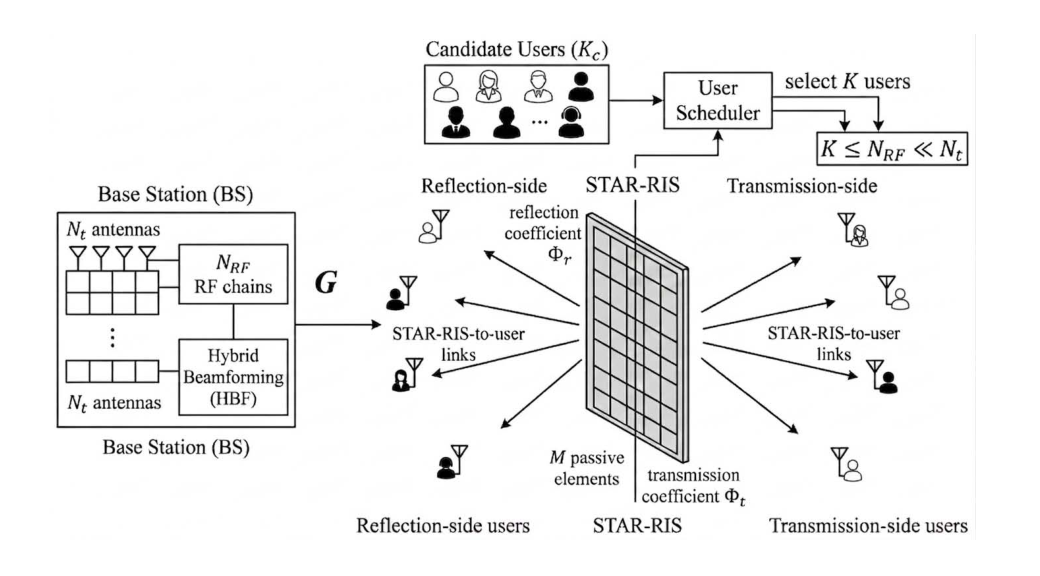
\includegraphics[width=0.78\textwidth,height=0.48\textheight,keepaspectratio]{ref_star_ris.pdf}\\[0.15em]
  {\scriptsize STAR-RIS architecture}\\[0.45em]
  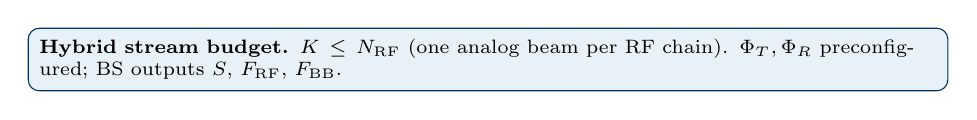
\begin{tikzpicture}
    \node[draw=navyblue, rounded corners, fill=softblue,
          align=left, inner sep=4pt, text width=0.94\textwidth, font=\scriptsize] {
      \textbf{Hybrid stream budget.}
      $K\le N_{\mathrm{RF}}$ (one analog beam per RF chain).
      $\Phi_T,\Phi_R$ preconfigured; BS outputs $S$, $F_{\mathrm{RF}}$, $F_{\mathrm{BB}}$.};
  \end{tikzpicture}\\[0.35em]
  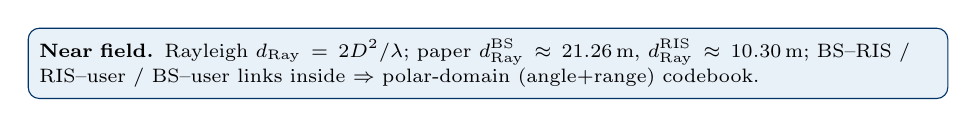
\begin{tikzpicture}
    \node[draw=navyblue, rounded corners, fill=softblue,
          align=left, inner sep=4pt, text width=0.94\textwidth, font=\scriptsize] {
      \textbf{Near field.}
      Rayleigh $d_{\mathrm{Ray}}=2D^2/\lambda$;
      paper $d_{\mathrm{Ray}}^{\mathrm{BS}}\approx 21.26$\,m, $d_{\mathrm{Ray}}^{\mathrm{RIS}}\approx 10.30$\,m;
      BS--RIS / RIS--user / BS--user links inside $\Rightarrow$ polar-domain (angle+range) codebook.};
  \end{tikzpicture}
\end{frame}
%======================================================================
% BRIDGE --- Three factors motivating Conflict Set
%======================================================================
\begin{frame}{3. Three Factors Aligned in $\eta_k$}
  \vspace{0.05cm}
  \begin{center}
  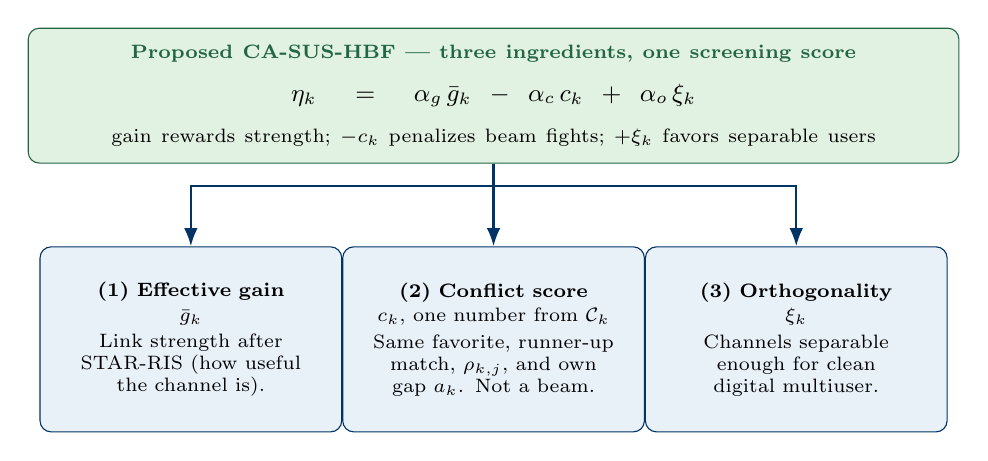
\begin{tikzpicture}[
      arr/.style={-{Latex}, thick, navyblue},
      card/.style={draw=navyblue, rounded corners, fill=softblue,
                   align=center, inner sep=4pt, font=\scriptsize,
                   text width=3.55cm, minimum height=2.35cm},
      etabox/.style={draw=notegreen, rounded corners, fill=softgreen,
                    align=center, inner sep=6pt}
    ]
    % TOP: overall idea + eta
    \node[etabox, text width=0.94\textwidth] (eta) {%
      {\scriptsize\color{notegreen}\textbf{Proposed CA-SUS-HBF --- three ingredients, one screening score}}\\[0.35em]
      {\small $\displaystyle\eta_k = \alpha_g\,\bar{g}_k - \alpha_c\,c_k + \alpha_o\,\xi_k$}\\[0.3em]
      {\scriptsize gain rewards strength; $-c_k$ penalizes beam fights; $+\xi_k$ favors separable users}};
    % BOTTOM: three equal ingredient cards
    \node[card, below=1.05cm of eta.south west, xshift=0.15cm, anchor=north west] (f1) {%
      \textbf{(1) Effective gain}\\[0.12em]
      $\bar{g}_k$\\[0.18em]
      Link strength after\\
      STAR-RIS (how useful\\
      the channel is).};
    \node[card, below=1.05cm of eta.south, anchor=north] (f2) {%
      \textbf{(2) Conflict score}\\[0.12em]
      $c_k$, one number from $\mathcal{C}_k$\\[0.18em]
      Same favorite, runner-up\\
      match, $\rho_{k,j}$, and own\\
      gap $a_k$. Not a beam.};
    \node[card, below=1.05cm of eta.south east, xshift=-0.15cm, anchor=north east] (f3) {%
      \textbf{(3) Orthogonality}\\[0.12em]
      $\xi_k$\\[0.18em]
      Channels separable\\
      enough for clean\\
      digital multiuser.};
    % idea -> ingredients
    \draw[arr] (eta.south) -- ++(0,-0.28) -| (f1.north);
    \draw[arr] (eta.south) -- (f2.north);
    \draw[arr] (eta.south) -- ++(0,-0.28) -| (f3.north);
  \end{tikzpicture}
  \end{center}
\end{frame}
%======================================================================
% FRAME --- Conflict set C_k + selection rule Gamma
%======================================================================
\begin{frame}{4. Who Conflicts ($\mathcal{C}_k$) and How $S$ Grows ($\Gamma$)}
  \vspace{-0.15cm}
  \begin{center}
  % --- Top: C_k ---
  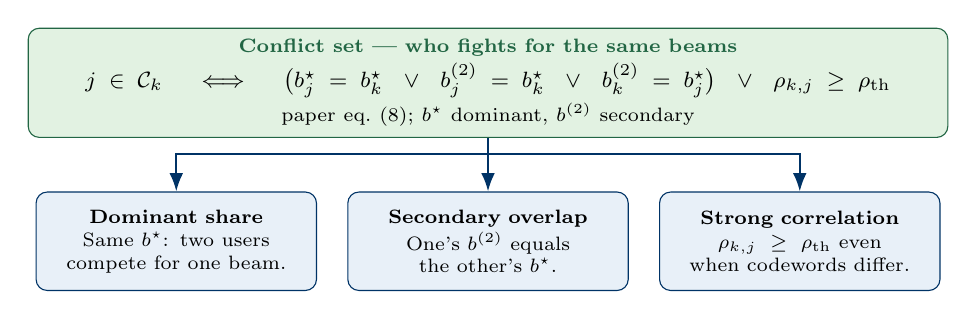
\begin{tikzpicture}[
      arr/.style={-{Latex}, thick, navyblue},
      eqbox/.style={draw=notegreen, rounded corners, fill=softgreen,
                    align=center, inner sep=4pt, font=\footnotesize},
      card/.style={draw=navyblue, rounded corners, fill=softblue,
                   align=center, inner sep=3pt, font=\scriptsize,
                   text width=3.35cm, minimum height=1.25cm}
    ]
    \node[eqbox, text width=0.94\textwidth] (eq) {%
      {\scriptsize\color{notegreen}\textbf{Conflict set --- who fights for the same beams}}\\[0.15em]
      $j\in\mathcal{C}_k
      \;\iff\;
      \bigl(
        b_j^\star = b_k^\star
        \;\vee\;
        b_j^{(2)} = b_k^\star
        \;\vee\;
        b_k^{(2)} = b_j^\star
      \bigr)
      \;\vee\;
      \rho_{k,j}\ge\rho_{\mathrm{th}}$\\[0.1em]
      {\scriptsize paper eq.~(8); $b^\star$ dominant, $b^{(2)}$ secondary}};
    \node[card, below=0.68cm of eq.south west, xshift=0.1cm, anchor=north west] (g1) {%
      \textbf{Dominant share}\\[0.08em]
      Same $b^\star$: two users\\
      compete for one beam.};
    \node[card, below=0.68cm of eq.south, anchor=north] (g2) {%
      \textbf{Secondary overlap}\\[0.08em]
      One's $b^{(2)}$ equals\\
      the other's $b^\star$.};
    \node[card, below=0.68cm of eq.south east, xshift=-0.1cm, anchor=north east] (g3) {%
      \textbf{Strong correlation}\\[0.08em]
      $\rho_{k,j}\ge\rho_{\mathrm{th}}$ even\\
      when codewords differ.};
    \draw[arr] (eq.south) -- ++(0,-0.2) -| (g1.north);
    \draw[arr] (eq.south) -- (g2.north);
    \draw[arr] (eq.south) -- ++(0,-0.2) -| (g3.north);
  \end{tikzpicture}\\[1em]
  % --- Bottom: Gamma ---
  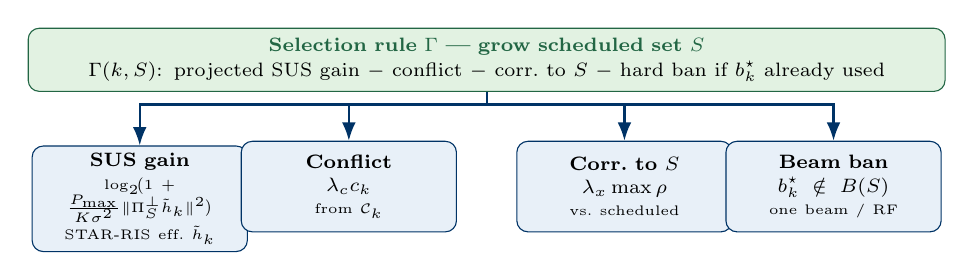
\begin{tikzpicture}[
      arr/.style={-{Latex}, thick, navyblue},
      eqbox/.style={draw=notegreen, rounded corners, fill=softgreen,
                    align=center, inner sep=3.5pt, font=\scriptsize},
      card/.style={draw=navyblue, rounded corners, fill=softblue,
                   align=center, inner sep=2.6pt, font=\scriptsize,
                   text width=2.55cm, minimum height=1.15cm}
    ]
    \node[eqbox, text width=0.94\textwidth] (gam) {%
      {\scriptsize\color{notegreen}\textbf{Selection rule $\Gamma$ --- grow scheduled set $S$}}\\[0.12em]
      $\Gamma(k,S)$: projected SUS gain
      $-$ conflict
      $-$ corr.\ to $S$
      $-$ hard ban if $b_k^\star$ already used};
    \node[card, below=0.68cm of gam.south west, xshift=0.05cm, anchor=north west] (f1) {%
  \textbf{SUS gain}\\[0.05em]
  {\tiny$\log_2\!\bigl(1+\tfrac{P_{\max}}{K\sigma^2}\|\Pi_S^\perp\tilde{h}_k\|^2\bigr)$}\\[0.05em]
  {\tiny STAR-RIS eff.\ $\tilde{h}_k$}};
    \node[card, below=0.62cm of gam, xshift=-1.75cm, anchor=north] (f2) {%
      \textbf{Conflict}\\[0.05em]
      $\lambda_c c_k$\\
      {\tiny from $\mathcal{C}_k$}};
    \node[card, below=0.62cm of gam, xshift=1.75cm, anchor=north] (f3) {%
      \textbf{Corr.\ to $S$}\\[0.05em]
      $\lambda_x\max\rho$\\
      {\tiny vs.\ scheduled}};
    \node[card, below=0.62cm of gam.south east, xshift=-0.05cm, anchor=north east] (f4) {%
      \textbf{Beam ban}\\[0.05em]
      $b_k^\star\notin B(S)$\\
      {\tiny one beam / RF}};
    \draw[arr] (gam.south) -- ++(0,-0.16) -| (f1.north);
    \draw[arr] (gam.south) -- ++(0,-0.16) -| (f2.north);
    \draw[arr] (gam.south) -- ++(0,-0.16) -| (f3.north);
    \draw[arr] (gam.south) -- ++(0,-0.16) -| (f4.north);
  \end{tikzpicture}\\[0.2em]
  {\scriptsize\textit{Classical SUS is codebook-blind; CA-SUS couples codebook conflict with channel orthogonality.}}
  \end{center}
\end{frame}
%======================================================================
% FRAME C --- Pipeline (4 breaths), sequential 1->2->3->4
%======================================================================
\begin{frame}{5. CA-SUS-HBF Pipeline}
  \vspace{0.05cm}
  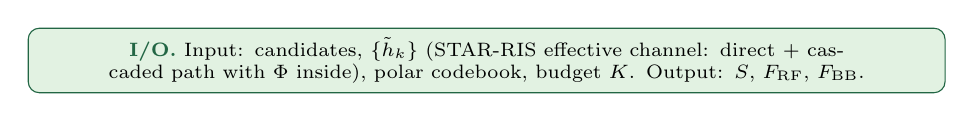
\begin{tikzpicture}
    \node[draw=notegreen, rounded corners, fill=softgreen,
          align=center, inner sep=3.5pt, text width=0.94\textwidth, font=\scriptsize] {
      \textbf{\color{notegreen}I/O.}
      Input: candidates, $\{\tilde{h}_k\}$ (STAR-RIS effective channel: direct + cascaded path with $\Phi$ inside), polar codebook, budget $K$.
      Output: $S$, $F_{\mathrm{RF}}$, $F_{\mathrm{BB}}$.};
  \end{tikzpicture}
  \vspace{0.25em}
  \begin{center}
  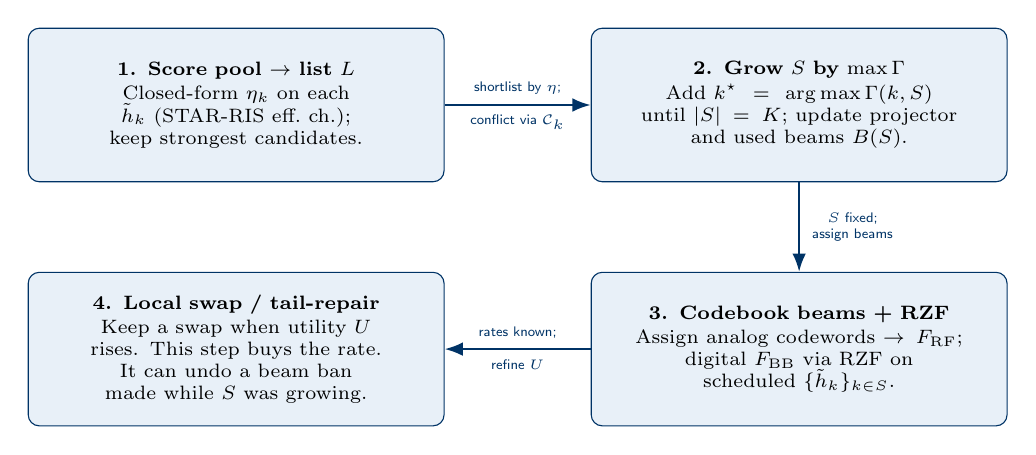
\begin{tikzpicture}[
      arr/.style={-{Latex}, thick, navyblue},
      card/.style={draw=navyblue, rounded corners, fill=softblue,
                   align=center, inner sep=4pt, font=\scriptsize,
                   text width=5.0cm, minimum height=1.95cm},
      lab/.style={font=\tiny\sffamily, text=navyblue, align=center}
    ]
    % Clockwise sequential: 1 -> 2 -> 3 -> 4
    \node[card] (c1) at (0,1.55) {%
      \textbf{1. Score pool $\to$ list $L$}\\[0.1em]
      Closed-form $\eta_k$ on each\\
      $\tilde{h}_k$ (STAR-RIS eff.\ ch.);\\
      keep strongest candidates.};
    \node[card] (c2) at (7.15,1.55) {%
      \textbf{2. Grow $S$ by $\max\Gamma$}\\[0.1em]
      Add $k^\star=\arg\max\Gamma(k,S)$\\
      until $|S|=K$; update projector\\
      and used beams $B(S)$.};
    \node[card] (c3) at (7.15,-1.55) {%
      \textbf{3. Codebook beams + RZF}\\[0.1em]
      Assign analog codewords $\to F_{\mathrm{RF}}$;\\
      digital $F_{\mathrm{BB}}$ via RZF on\\
      scheduled $\{\tilde{h}_k\}_{k\in S}$.};
    \node[card] (c4) at (0,-1.55) {%
      \textbf{4. Local swap / tail-repair}\\[0.1em]
      Keep a swap when utility $U$\\
      rises. This step buys the rate.\\
      It can undo a beam ban\\
      made while $S$ was growing.};
    % 1 -> 2
    \draw[arr] (c1.east) -- node[lab, above] {shortlist by $\eta$;} node[lab, below] {conflict via $\mathcal{C}_k$} (c2.west);
    % 2 -> 3
    \draw[arr] (c2.south) -- node[lab, right, xshift=1pt] {$S$ fixed;\\assign beams} (c3.north);
    % 3 -> 4
    \draw[arr] (c3.west) -- node[lab, above] {rates known;} node[lab, below] {refine $U$} (c4.east);
  \end{tikzpicture}
  \end{center}
\end{frame}
%======================================================================
% CHANGE --- what to edit in the scheduler
% Numbers above this frame are the submitted method. Do not reuse them here.
%======================================================================

%======================================================================
% RESULTS --- Rate
%======================================================================
\begin{frame}{6. Simulation Results (Rate)}
  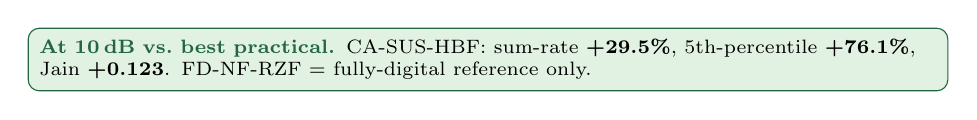
\begin{tikzpicture}
    \node[draw=notegreen, rounded corners, fill=softgreen,
          align=left, inner sep=4pt, text width=0.94\textwidth, font=\scriptsize] {
      \textbf{\color{notegreen}At 10\,dB vs.\ best practical.}
      CA-SUS-HBF: sum-rate \textbf{+29.5\%}, 5th-percentile \textbf{+76.1\%}, Jain \textbf{+0.123}.
      FD-NF-RZF = fully-digital reference only.};
  \end{tikzpicture}
  \vspace{0.2em}
  \begin{columns}[T,onlytextwidth]
    \begin{column}{0.49\textwidth}
      \centering
      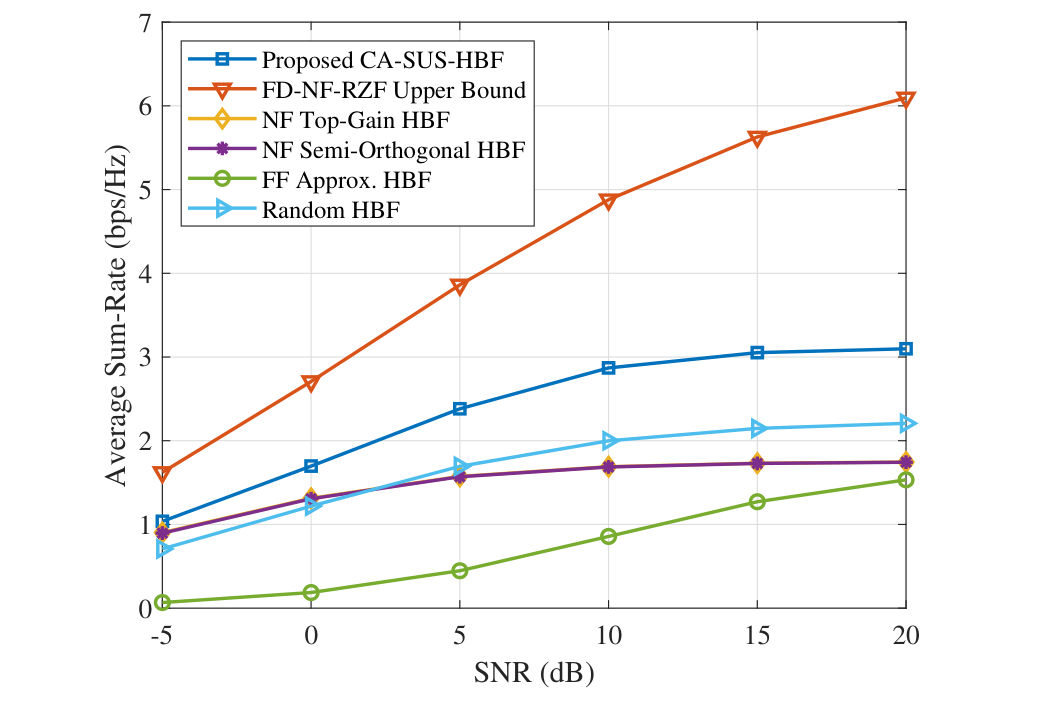
\includegraphics[width=\linewidth,height=0.48\textheight,keepaspectratio]{fig1.pdf}\\[0.15em]
      {\scriptsize Fig.~1. Average sum-rate versus SNR for different hybrid beamforming schemes.}
    \end{column}
    \begin{column}{0.49\textwidth}
      \centering
      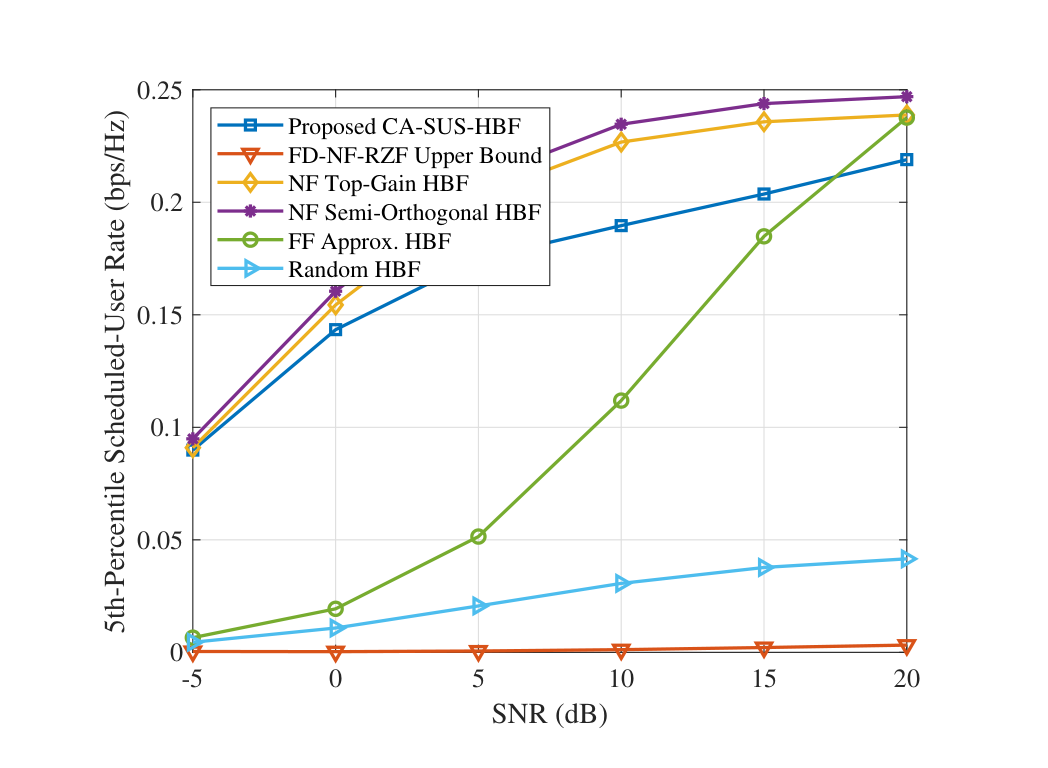
\includegraphics[width=\linewidth,height=0.48\textheight,keepaspectratio]{fig2.pdf}\\[0.15em]
      {\scriptsize Fig.~2. 5th-percentile scheduled-user rate versus SNR.}
    \end{column}
  \end{columns}
\end{frame}
%======================================================================
% RESULTS --- Users / Fairness
%======================================================================
\begin{frame}{7. Simulation Results (Users and Rate--Fairness)}
  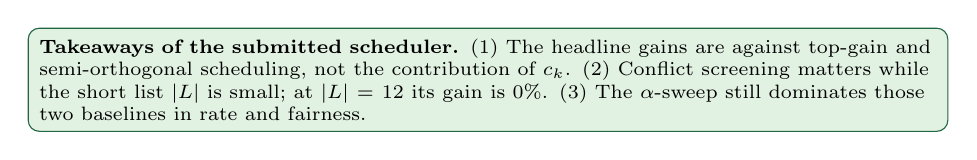
\begin{tikzpicture}
    \node[draw=notegreen, rounded corners, fill=softgreen,
          align=left, inner sep=4pt, text width=0.94\textwidth, font=\scriptsize] {
      \textbf{Takeaways of the submitted scheduler.}
      (1)~The headline gains are against top-gain and semi-orthogonal scheduling, not the contribution of $c_k$.
      (2)~Conflict screening matters while the short list $|L|$ is small; at $|L|=12$ its gain is 0\%.
      (3)~The $\alpha$-sweep still dominates those two baselines in rate and fairness.};
  \end{tikzpicture}
  \vspace{0.2em}
  \begin{columns}[T,onlytextwidth]
    \begin{column}{0.49\textwidth}
      \centering
      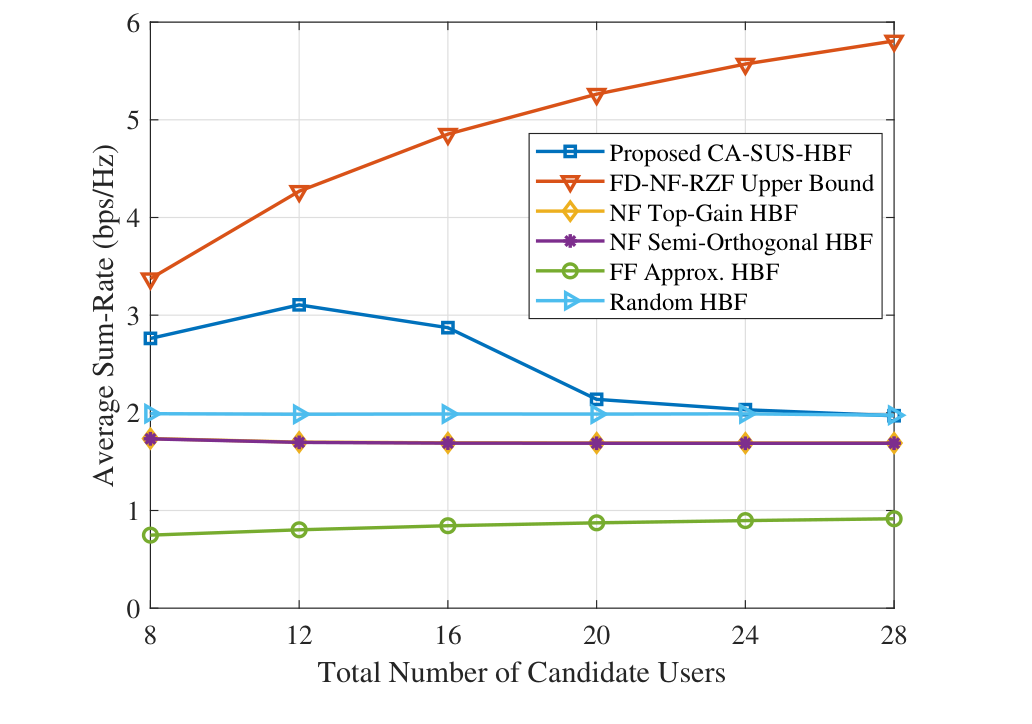
\includegraphics[width=\linewidth,height=0.48\textheight,keepaspectratio]{fig3.pdf}\\[0.15em]
      {\scriptsize Fig.~3. Average sum-rate versus the total number of candidate users.}
    \end{column}
    \begin{column}{0.49\textwidth}
      \centering
      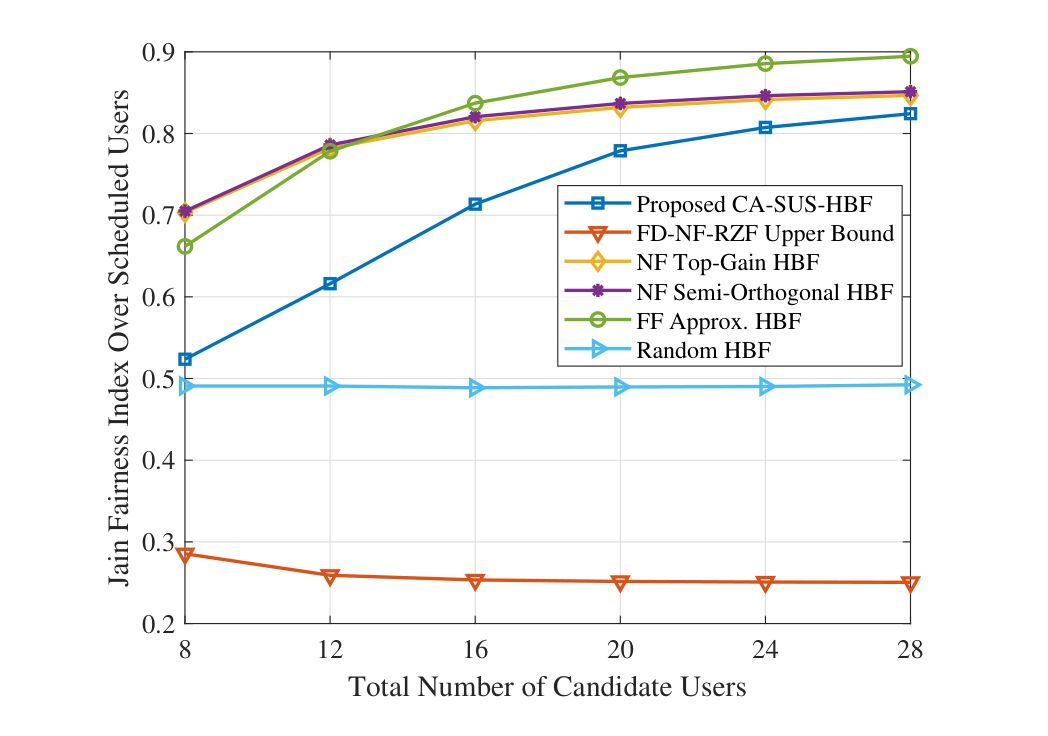
\includegraphics[width=\linewidth,height=0.48\textheight,keepaspectratio]{fig4.pdf}\\[0.15em]
      {\scriptsize Fig.~4. Throughput--fairness region obtained by sweeping $\alpha$.}
    \end{column}
  \end{columns}
\end{frame}
%======================================================================
% REFERENCES
%======================================================================
\begin{frame}[t]{8. References}
\vspace{-0.8em}

\fontsize{6.0pt}{6.2pt}\selectfont
\begin{thebibliography}{20}
%\setlength{\itemsep}{0.05em}
\setlength{\parsep}{0pt}
\setlength{\parskip}{0pt}
\bibitem{guirado}
R.~Guirado, R.~Verdecia-Pe\~{n}a, G.~Perez-Palomino, E.~Carrasco, and J.~I.~Alonso,
``Prototype and performance assessment of mmWave active RIS-enhanced 6G wireless communications,''
\textit{IEEE Trans.\ Green Commun.\ Netw.}, vol.~10, pp.~412--425, 2026.
\bibitem{wu_zhang_irs}
Q.~Wu and R.~Zhang,
``Intelligent reflecting surface enhanced wireless network via joint active and passive beamforming,''
\textit{IEEE Trans.\ Wireless Commun.}, vol.~18, no.~11, pp.~5394--5409, 2019.
\bibitem{mu_star}
X.~Mu, Y.~Liu, L.~Guo, J.~Lin, and R.~Schober,
``Simultaneously transmitting and reflecting (STAR) RIS aided wireless communications,''
\textit{IEEE Trans.\ Wireless Commun.}, vol.~21, no.~5, pp.~3083--3098, 2022.
\bibitem{khalid}
W.~Khalid, Z.~Kaleem, R.~Ullah, T.~Van Chien, S.~Noh, and H.~Yu,
``Simultaneous transmitting and reflecting-reconfigurable intelligent surface in 6G: Design guidelines and future perspectives,''
\textit{IEEE Netw.}, vol.~37, no.~5, pp.~173--181, 2023.
\bibitem{ayach}
O.~E.~Ayach, S.~Rajagopal, S.~Abu-Surra, Z.~Pi, and R.~W.~Heath,
``Spatially sparse precoding in millimeter wave MIMO systems,''
\textit{IEEE Trans.\ Wireless Commun.}, vol.~13, no.~3, pp.~1499--1513, 2014.
\bibitem{molisch}
A.~F.~Molisch, V.~V.~Ratnam, S.~Han, Z.~Li, S.~L.~H.~Nguyen, L.~Li, and K.~Haneda,
``Hybrid beamforming for massive MIMO: A survey,''
\textit{IEEE Commun.\ Mag.}, vol.~55, no.~9, pp.~134--141, 2017.
\bibitem{dao}
H.~T.~Dao and S.~Kim,
``Effective channel gain-based access point selection in cell-free massive MIMO systems,''
\textit{IEEE Access}, vol.~8, pp.~108127--108132, 2020.
\bibitem{mao_sus}
J.~Mao, J.~Gao, Y.~Liu, and G.~Xie,
``Simplified semi-orthogonal user selection for MU-MIMO systems with ZFBF,''
\textit{IEEE Wireless Commun.\ Lett.}, vol.~1, no.~1, pp.~42--45, 2012.
\bibitem{yoo}
T.~Yoo and A.~Goldsmith,
``On the optimality of multiantenna broadcast scheduling using zero-forcing beamforming,''
\textit{IEEE J.\ Sel.\ Areas Commun.}, vol.~24, no.~3, pp.~528--541, 2006.
\bibitem{wu_zhang_env}
Q.~Wu and R.~Zhang,
``Towards smart and reconfigurable environment: Intelligent reflecting surface aided wireless network,''
\textit{IEEE Commun.\ Mag.}, vol.~58, no.~1, pp.~106--112, 2020.
\bibitem{alkhateeb}
A.~Alkhateeb, O.~El~Ayach, G.~Leus, and R.~W.~Heath,
``Channel estimation and hybrid precoding for millimeter wave cellular systems,''
\textit{IEEE J.\ Sel.\ Topics Signal Process.}, vol.~8, no.~5, pp.~831--846, 2014.
\bibitem{cui_dai}
M.~Cui and L.~Dai,
``Near-field wideband beamforming for extremely large antenna arrays,''
\textit{IEEE Trans.\ Wireless Commun.}, vol.~23, no.~10, pp.~13110--13124, 2024.
\end{thebibliography}
\end{frame}
\begin{frame}[plain]
\begin{tikzpicture}[remember picture, overlay]
    \fill[navyblue] (current page.south west) rectangle (current page.north east);
\end{tikzpicture}
\vspace{1.5cm}
\begin{center}
    \textcolor{white}{\Huge\textbf{Thank You}}\\[0.8cm]
    \textcolor{white}{\small \confshort~$\bullet$~Quy Nhon}\\[0.45cm]
    %\textcolor{white}{\footnotesize 24100706@st.phenikaa-uni.edu.vn}
\end{center}
\end{frame}
\end{document}
